\documentclass[aspectratio=169]{beamer}

\usepackage{amsthm}
\usepackage{amssymb}
\usepackage{amsfonts}
\usepackage{amsmath}
\usepackage{mathtools}

\usepackage{pgf}
\usepgflibrary{fpu}
\usepackage{pgfplots}
\usepackage{tikz}
\usetikzlibrary{angles,fit,arrows,calc,math,matrix,intersections,through,backgrounds,cd}
\usepackage{tkz-euclide}
\usepackage{tkz-graph}
\usepackage{graphicx}
\pgfplotsset{compat=1.18}

\usetheme{Pittsburgh}
\usecolortheme{seahorse}

\title{Arithmetic expression geometry}
\author[Author] {Mingli Yuan}

\begin{document}
\pgfplotsset{compat=1.18}

\begin{frame}
\maketitle
\end{frame}

\begin{frame}
\frametitle{Table of Contents}
\tableofcontents
\end{frame}

\section{Prelude}

\begin{frame}
\frametitle{Universality}
\emph{E pluribus unum: From Complexity, Universality} by Terence Tao
\begin{itemize}
    \item the law of large numbers
    \item the central limit theorem
\end{itemize}
\begin{figure}[ht]\centering
\resizebox{0.3\textwidth}{!}{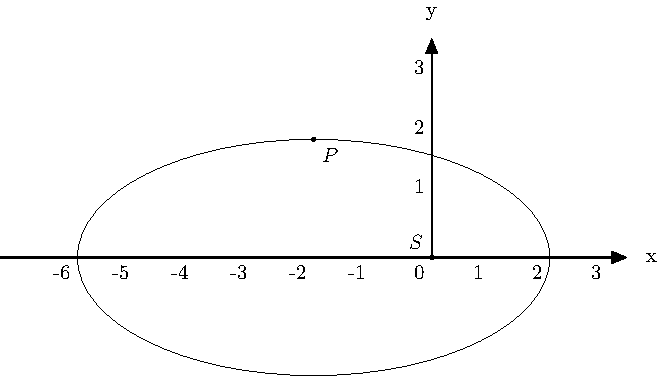
\includegraphics{images/2body}}
\resizebox{0.3\textwidth}{!}{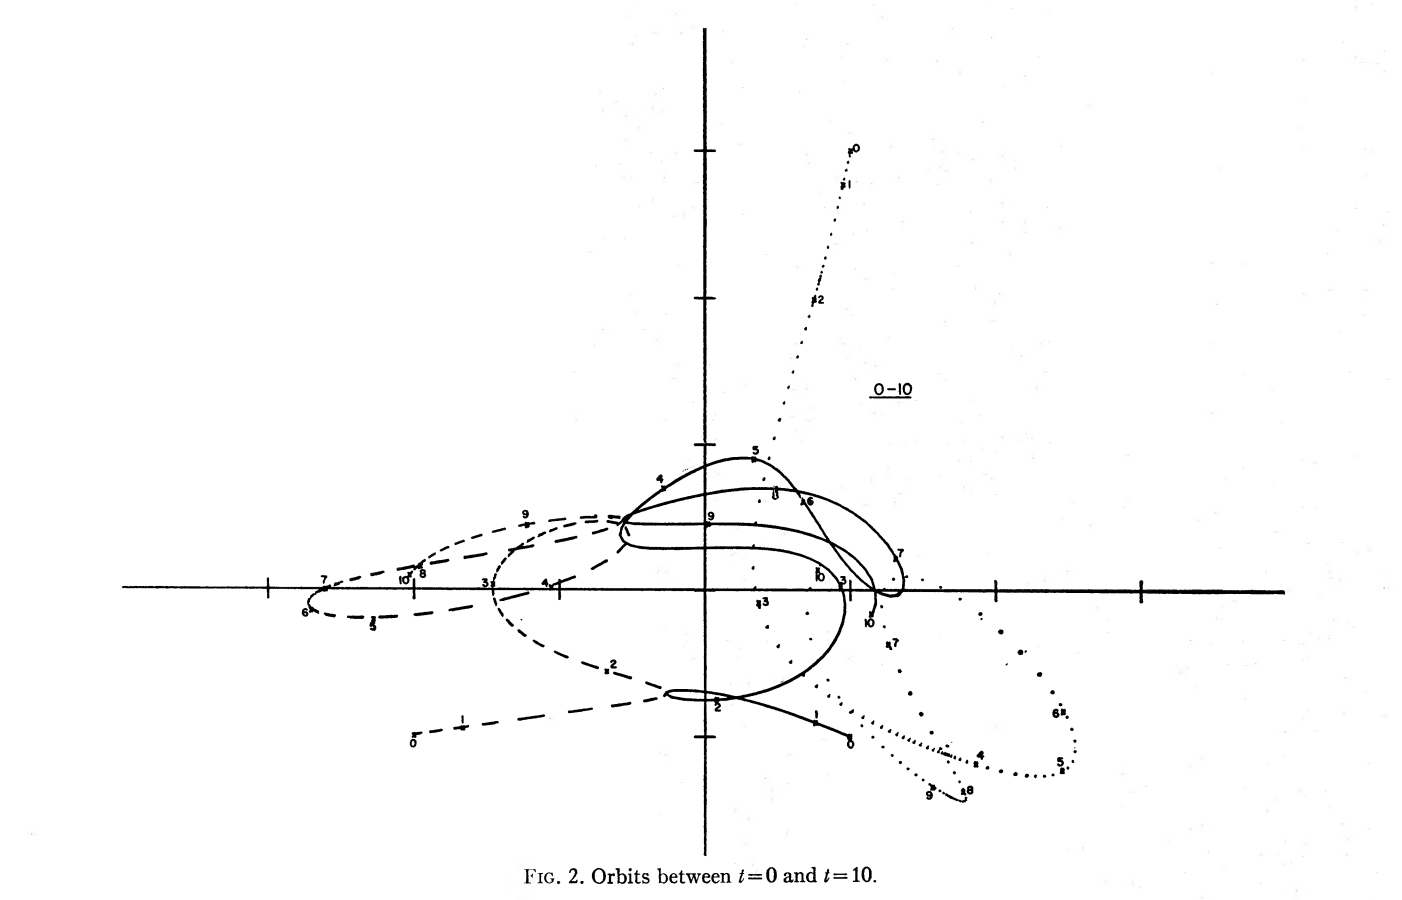
\includegraphics{images/3body}}
\resizebox{0.3\textwidth}{!}{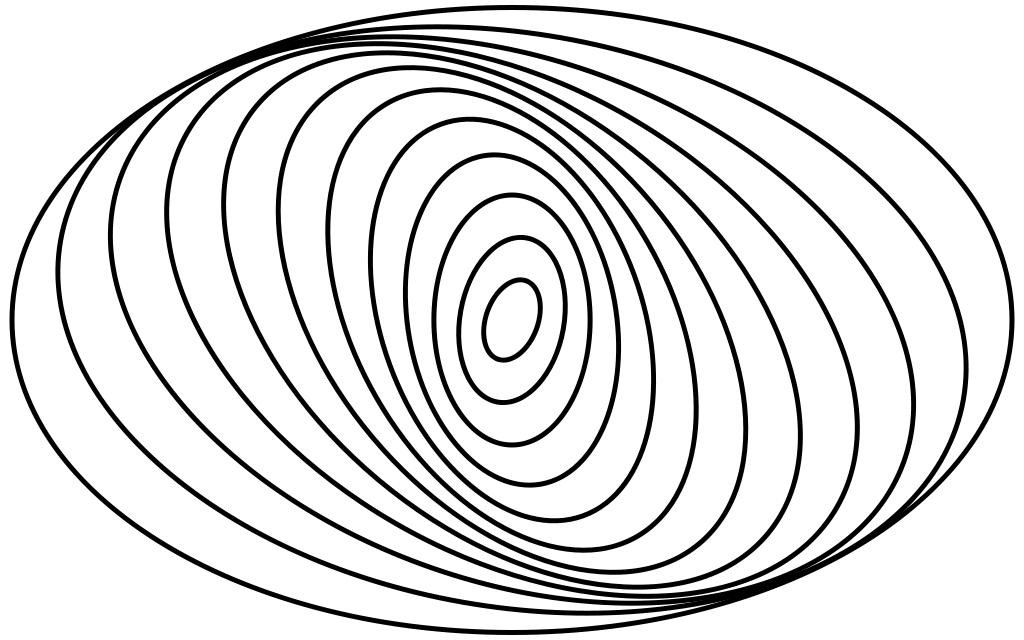
\includegraphics{images/spiral_galaxy_arms_diagram}}
\caption{a 2-body orbit; a 3-body orbit; dense wave of spiral galaxies}
\end{figure}
\end{frame}

\begin{frame}
\frametitle{Overparameterization}
\end{frame}

\begin{frame}
\frametitle{Expressiveness of dimensions}

\end{frame}

\begin{frame}
\frametitle{A neglected possibility}
\end{frame}

\begin{frame}
\frametitle{Random walks}
\end{frame}

\begin{frame}
\frametitle{Relation and parallelism}
\end{frame}

\begin{frame}
\frametitle{But how?}
\end{frame}

\end{document}
